\documentclass{article}
\usepackage[final]{neurips_2026}
\usepackage[utf8]{inputenc}
\usepackage[T1]{fontenc}
\usepackage{hyperref}
\hypersetup{hidelinks}
\usepackage{url}
\usepackage{booktabs}
\usepackage{amsfonts}
\usepackage{amsmath}
\usepackage{graphicx}
\usepackage{microtype}
\usepackage{xcolor}
\usepackage{float}
\usepackage{enumitem}
\usepackage{array}
\setlist[itemize]{leftmargin=12pt,itemsep=1pt,topsep=2pt}

\title{Predicting Injury-Producing NYC Motor Vehicle Collisions\\Using Multi-Table Crash, Vehicle, and Person Data}

\author{Alan Nemkovsky \\
Section ID: 05 \\
NetID: an1078}

\begin{document}
\maketitle

\begin{abstract}
This project studies whether injury-producing motor vehicle collisions in New York City can be predicted from linked public crash, vehicle, and person records. Using NYC Motor Vehicle Collisions data, I construct a crash-level binary target for whether at least one injury or fatality occurred, aggregate vehicle and person rows to the collision level, exclude direct outcome fields to reduce leakage, and compare logistic regression, random forest, extra trees, and XGBoost under a temporal split that trains on 2021 to 2024 collisions and tests on 2025 collisions. The best model was XGBoost, with ROC-AUC 0.893, PR-AUC 0.860, F1 0.787, precision 0.742, and recall 0.839 on 85,543 held-out 2025 collisions. Ablation analysis showed that adding linked vehicle and person information improved PR-AUC from 0.656 with crash-only features to 0.846 with the full leakage-controlled feature set. 
\\Code: \url{https://github.com/AlanNemkovsky/NYC-Collision-Final-Project}. 
\\Video: \url{https://drive.google.com/file/d/1Ck1Ilf0Wi1tFBWO5ak2oMGRYA9pWlKzK/view?usp=sharing}.
\end{abstract}

\section{Introduction}
Collision deaths in large cities like New York City (NYC) are a major public safety issue. NYC’s data-driven traffic safety program publishes large data collections of motor vehicle collision (MVC) records. The New York City Department of Transportation (NYC DOT) reports that traffic deaths in 2025 were the fewest ever recorded in the city, with 205 traffic fatalities, which represents a 19 percent decrease in traffic deaths from 2024 \citep{nyc_dot_2026}. Despite the reduction in traffic fatalities, MVCs still have a significant social cost to society.

The main question that will be explored in this project is whether a motor vehicle collision can be classified as injury-producing based on information recorded in three different NYC Motor Vehicle Collisions tables. An injury-producing collision is defined as a collision in which at least one person involved in the MVC was injured or killed as a result of the collision. While this project will analyze the listed features of each MVC, it will not attempt to determine whether any of those listed features are the cause of injuries in those MVCs.

In this project, four main results will be presented. First, a data analysis pipeline will be created that audits the more than twelve million raw data rows from the three NYC MVC CSV files to create a new table containing the information that can be used to build models to predict whether each MVC was injury-producing. Second, methods will be implemented to ensure that there is no leakage of information from the outcome variable of injury-producing MVCs into the model by excluding information on the injuries or fatalities in those MVCs from the features used to create classification models. Third, classification models will be implemented and compared using the 2025 MVC data as a test set. Finally, an analysis of the data using principal component analysis and K-Means clustering will be performed to gain additional insights into the data. This project offers more information than the analysis of the MVC tables as a whole because this analysis includes assessing the added value of the vehicle and person tables to the outcome of the MVCs.

\section{Related work}

Crash injury severity is a common prediction task due to the influence of various factors on the injury severity of those involved in a crash. A recent review of the use of machine learning techniques for the task of crash injury severity prediction indicates that methods like random forests, support vector machines, and decision trees have been effective at performing the prediction, though often with concerns regarding validity of the models \citep{santos2022review}. In this project, random forests, extra trees, gradient boosting, and logistic regression will be used to attempt to appropriately model the severity of crashes. Logistic regression models can be used to provide interpretability to the model, while random forests, extra trees, and gradient boosting models can be used to model nonlinear interactions between the various variables.

The data is obtained from the New York City crash table, which contains one row per crash, the vehicle table which contains one row per vehicle involved in a crash, and the person table which contains one row per person involved in a crash. New York City made available in one of their reports that the crash table is based upon police reported collisions, the vehicle table reports on each vehicle involved in the collision, and the person table reports on each person involved in the collision \citep{nyc_crashes,nyc_vehicles,nyc_person}. These tables can be used in a relational data science workflow due to the shared \texttt{COLLISION\_ID} of each table. However, using the variables related to the injury of each person involved in the crash as the target variable for prediction is invalid, as these variables are the target that defines whether there was an injury in the crash after it occurred. Thus, such variables must be processed during construction of the model.

\section{Data}
The raw inputs are three local CSV files downloaded from NYC Open Data: \path{Motor_Vehicle_Collisions_-_Crashes.csv}, \path{Motor_Vehicle_Collisions_-_Vehicles.csv}, and \path{Motor_Vehicle_Collisions_-_Person.csv}. The raw audit found 2,257,882 crash rows, 4,528,736 vehicle rows, and 5,945,665 person rows. All three files contained a detectable \texttt{COLLISION\_ID} field. The cleaned feature matrix was restricted to records from 2021 onward and contained 513,035 collision-level rows and 94 columns. The overall injury-or-fatality target rate in this cleaned matrix was 40.2 percent.

\begin{table}[H]
\centering
\caption{Dataset summary after cleaning and aggregation. The model table keeps one row per collision and aggregates linked vehicle and person records by \texttt{COLLISION\_ID}.}
\small
\begin{tabular}{lr}
\toprule
Metric & Value \\
\midrule
Collision-level rows used for modeling & 513,035 \\
Feature matrix columns & 94 \\
Target positive rate & 0.402 \\
Minimum crash year & 2021 \\
Maximum crash year in cleaned data & 2026 \\
Mean vehicle records per collision & 2.018 \\
Mean person records per collision & 3.474 \\
Training rows, 2021 to 2024 & 402,367 \\
Held-out test rows, 2025 & 85,543 \\
\bottomrule
\end{tabular}
\end{table}

The crash table provided the target and basic context: crash date, crash time, borough, ZIP code, latitude, longitude, street fields, contributing factors, vehicle type codes, and injury/fatality counts. The vehicle table added vehicle state, type, year, travel direction, pre-crash movement, point of impact, public property damage flags, and additional contributing factors. The person table added person type, role, age, sex, seating position, safety equipment, and pedestrian action/location fields. Because the modeling unit is the collision, vehicle and person records were aggregated into counts, indicators, shares, and summary statistics.

\section{Method}
\subsection{Cleaning and feature construction}
The audit pipeline begins with an audit of the data to determine its schema, row counts, missing values, duplicates, and integrity. The data is standardized to have consistent column names, crash dates are parsed for date and time components, crash labels are lowercased, injury and fatality counts are converted to numeric values, age and vehicle-year counts are cleaned, and the data is filtered to only include crashes that occurred between the years of 2021 and 2026. Years 2021 to 2024 are used to train the model, 2025 is used to evaluate the model performance on held-out data, and 2026 is not used in testing to account for the fact that it is a slice of future data included in the downloaded data file.

Several groups of features are engineered for the crash prediction model.  Crash features include variables related to the crash itself, such as the borough in which the crash occurred, the ZIP-code in which the crash occurred, the latitude and longitude of the crash, the time of the crash (hour of the day, weekday of the crash, month of the crash, whether the crash occurred on a weekend, whether it occurred during rush-hour, late at night, on a street, and the contributing factors to the crash.  Vehicle features include variables related to the vehicles involved in the crash, such as the number of vehicle records related to the crash, the type of each of those vehicles, the number of commercial vehicles involved in the crash, the number of heavy vehicles involved in the crash, the number of taxis, buses, bikes, motorcycles, and trucks involved in the crash, and the actions that each of those vehicles was performing prior to the crash.  Finally, person-related features include variables related to each of the individuals involved in the crash, such as the number of individuals involved in the crash, the number of each type of individuals involved (drivers, pedestrians, bicyclists), the sex of each of those individuals, the age of those individuals, the role of each of those individuals in relation to the crash, the use of safety equipment by those individuals, and the actions performed by each of those individuals prior to the crash.

\subsection{Leakage control}

Another design decision that was made was to avoid outcome leakage. The target for the model is based upon the number of injuries and fatalities from each crash, but those fields are removed from the feature matrix that is provided to the model. Additionally, any fields related to the individuals involved in the crashes, such as \texttt{PERSON\_INJURY}, \texttt{BODILY\_INJURY}, \texttt{COMPLAINT}, \texttt{EJECTION}, and \texttt{EMOTIONAL\_STATUS} are also excluded from the feature matrix. Finally, fields related to the raw names of the streets and the times of the crashes in their raw string form are also removed from the model, although factors like the time of day when the crashes occurred are included. Thus, each of these choices helps to ensure that the results of the model are more defensible as a model that classifies the severity of crashes.

\subsection{Models and evaluation}
The task to be performed is binary classification. The split to be used is temporal, splitting the data according to whether the collisions occurred before or after 2025. Each of these splits is more stringent than a random split, as it evaluates the model’s ability to generalize its findings from an earlier year to a later year. The models to be used include a dummy classifier that selects the most frequent class, logistic regression with regularization, random forest classifiers, extra trees classifiers, and optionally XGBoost classifiers \citep{breiman2001random,xgboost,sklearn}. For each of these models, the following metrics will be calculated: ROC-AUC, PR-AUC, accuracy, balanced accuracy, precision, recall, and F1 scores. Since the positive class is large but not dominant within the classes, the precision and recall scores will be emphasized. Furthermore, the threshold will be optimized on the training set to maximize the F1 score, and that same threshold will be applied to the 2025 data.

\section{Evaluation and results}
\subsection{Exploratory findings}

The table of model coefficients and associated statistics indicates that the share of collisions that resulted in injuries rose from 35.1 percent in 2021 to 44.1 percent in 2024, and remained high at 43.7 percent in the test year of 2025. While this contradicts the city’s declining rate of traffic fatalities, this statistic is not contradictory to those traffic fatality results; the target variable includes both the fatalities and injuries from traffic collisions, and reports the number of collisions that resulted in at least one fatality or injury (as a share of the total number of reported traffic collisions). The most common contributing factor to traffic collisions was the factor of the inattention or distraction of the driver, which was listed in 148,410 of the reported traffic collisions in the data set. Other common contributing factors to traffic collisions included the factors of traveling too closely behind another vehicle, failing to yield the right-of-way to another vehicle, passing or using lanes in an improper manner, other vehicular issues, traveling at an unsafe speed, and disregarding traffic control measures.

\begin{figure}[H]
\centering
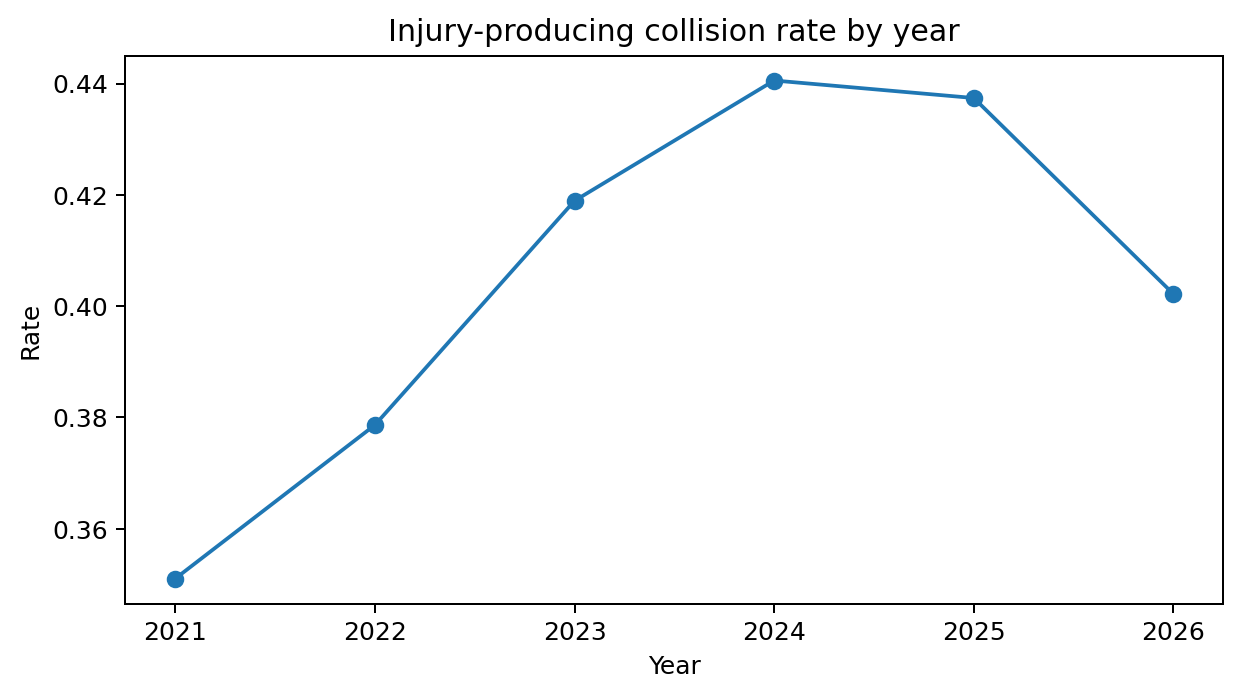
\includegraphics[width=0.48\linewidth]{figures/fig_injury_rate_by_year.png}\hfill
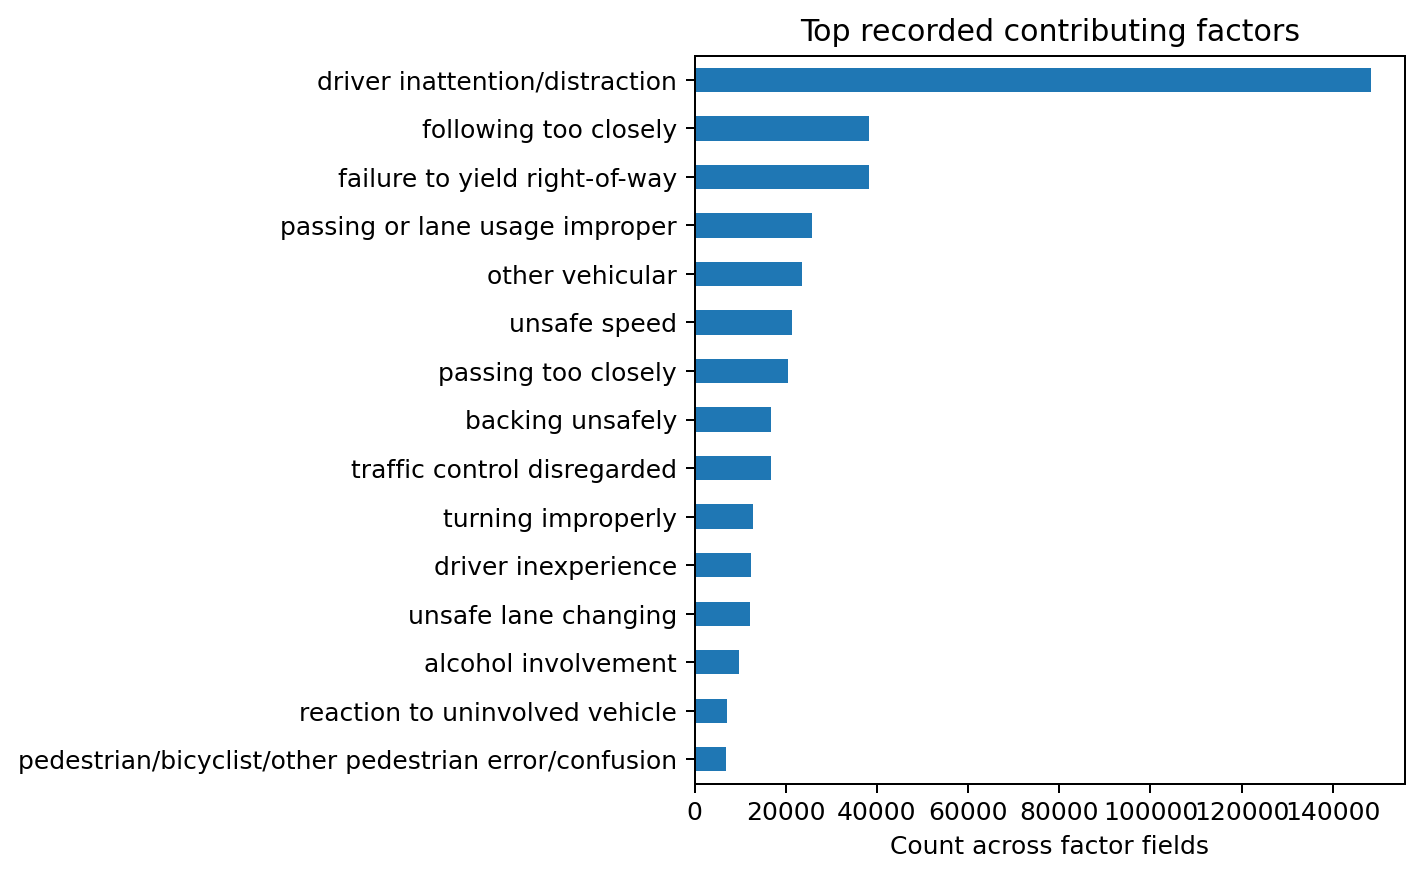
\includegraphics[width=0.48\linewidth]{figures/fig_top_factors.png}
\caption{Exploratory results. Left: the injury-or-fatality share among reported collisions increased from 2021 to 2024 and stayed high in 2025. Right: driver inattention/distraction was the dominant contributing factor in the cleaned records.}
\end{figure}

The number and type of linked records also matter. Collisions with only one vehicle have a higher share of injuries than collisions between two vehicles - there are many one-vehicle collisions with pedestrians and cyclists, for example. Additionally, the share of collisions with injuries increases with the number of people records in each collision, as one would expect for collisions involving more people. Thus, these metrics support the use of the linked person and vehicle aggregate records rather than the crash table alone.

\begin{figure}[H]
\centering
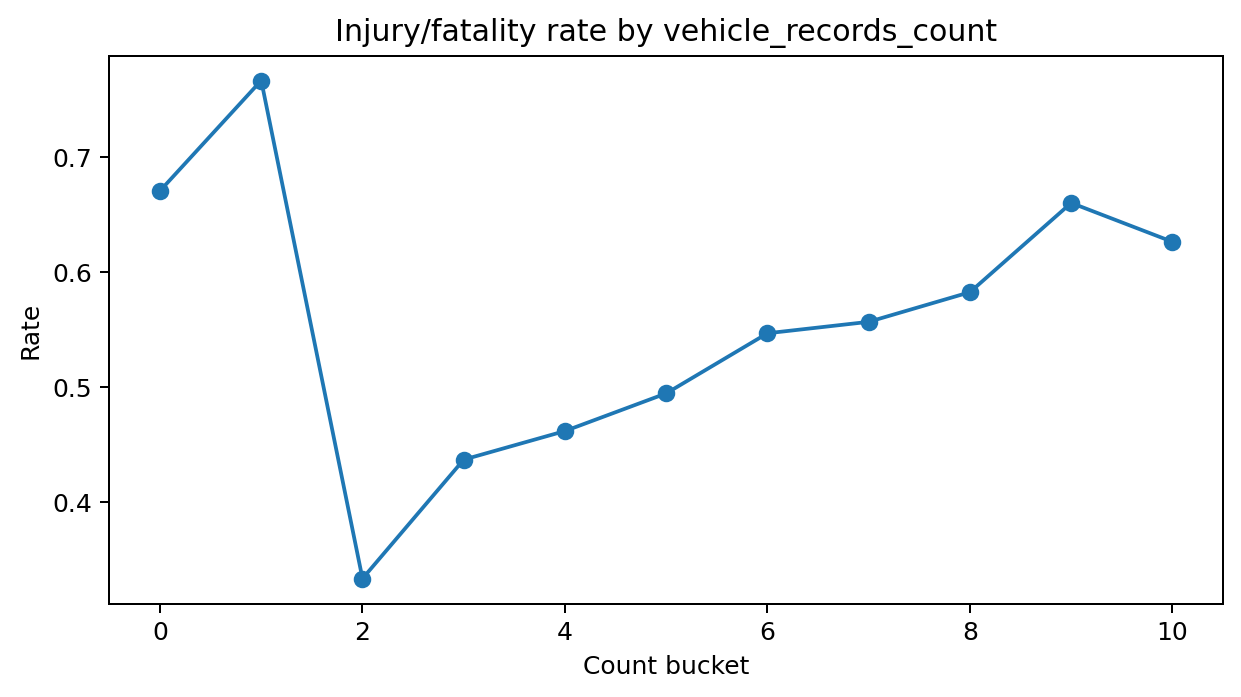
\includegraphics[width=0.48\linewidth]{figures/fig_injury_rate_by_involvement.png}\hfill
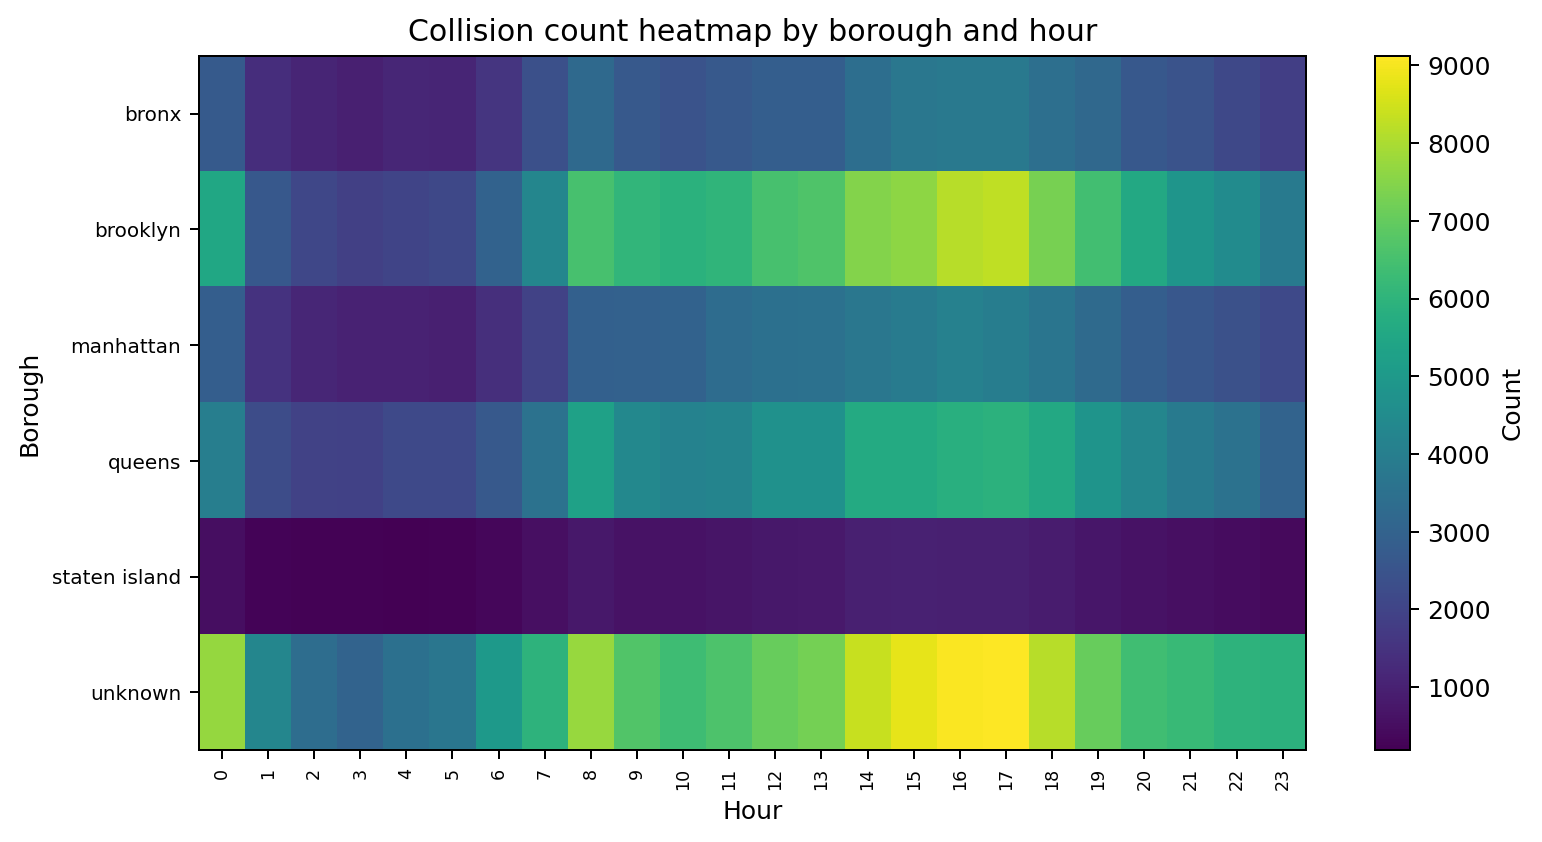
\includegraphics[width=0.48\linewidth]{figures/fig_borough_hour_heatmap.png}
\caption{Multi-table context. Left: injury rate varies sharply with the number of linked vehicle and person records. Right: crash volume by borough and hour shows strong temporal and spatial structure.}
\end{figure}

\subsection{Predictive performance}
The best performing model using the PR-AUC metric was the XGBoost model. It achieved a ROC-AUC of 0.893, a PR-AUC of 0.860, accuracy of 0.802, a balanced accuracy of 0.806, precision of 0.742, a recall of 0.839, and an F1 score of 0.787 on the 2025 test set. The random forest, logistic regression, and extra trees models were all close behind in performance to the XGBoost model. The regularized logistic regression model achieved a PR-AUC of 0.846 and a ROC-AUC of 0.885, indicating that the engineered features for the model already contain a linear signal. Finally, the gap between the baseline model with dummy scores and the learned models indicates that the task is learnable from the linked administrative data.

\begin{table}[H]
\centering
\caption{Held-out 2025 model performance. XGBoost performs best by PR-AUC, while logistic regression remains competitive and more interpretable.}
\small
\begin{tabular}{lrrrrrr}
\toprule
Model & Accuracy & Bal. Acc. & Precision & Recall & F1 & PR-AUC \\
\midrule
XGBoost & 0.802 & 0.806 & 0.742 & 0.839 & 0.787 & 0.860 \\
Random forest & 0.798 & 0.801 & 0.742 & 0.825 & 0.781 & 0.853 \\
Logistic L2 & 0.797 & 0.800 & 0.743 & 0.820 & 0.780 & 0.846 \\
Extra trees & 0.790 & 0.793 & 0.737 & 0.810 & 0.772 & 0.841 \\
Dummy baseline & 0.437 & 0.500 & 0.437 & 1.000 & 0.609 & 0.437 \\
\bottomrule
\end{tabular}
\end{table}

\begin{figure}[H]
\centering
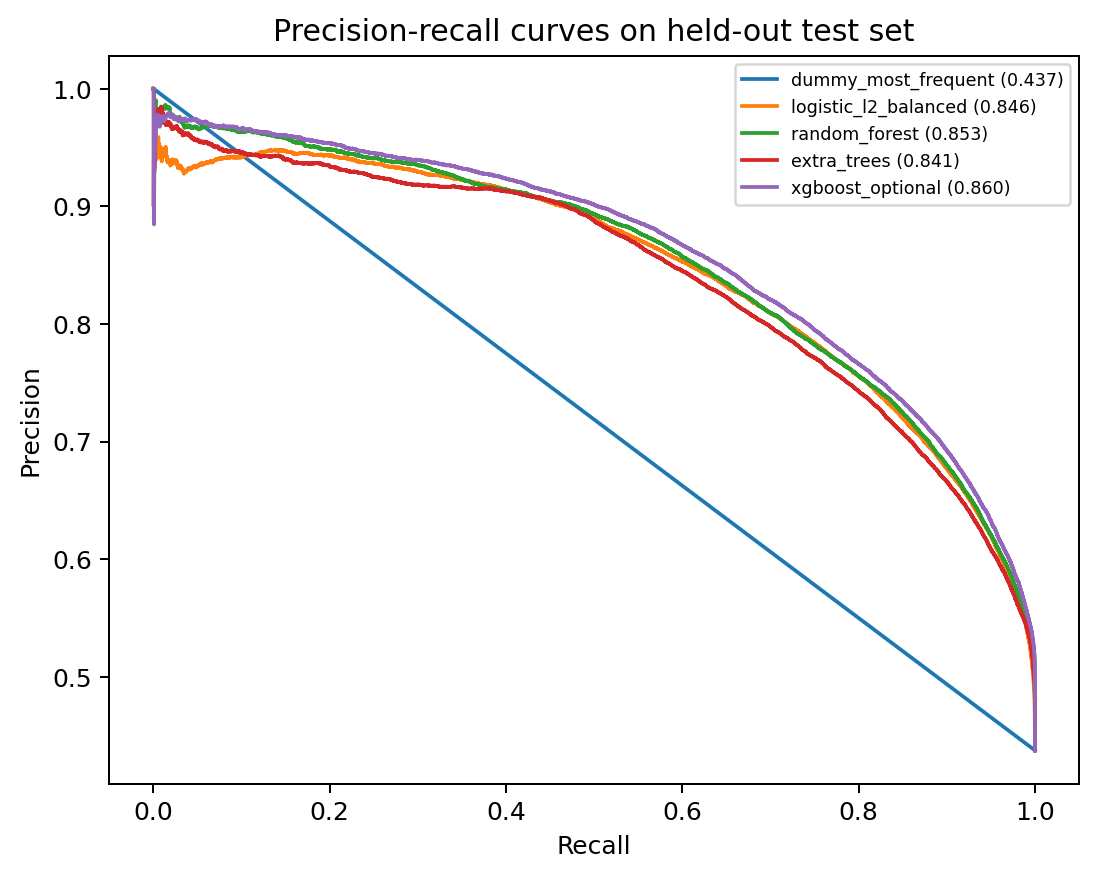
\includegraphics[width=0.48\linewidth]{figures/fig_pr_curves.png}\hfill
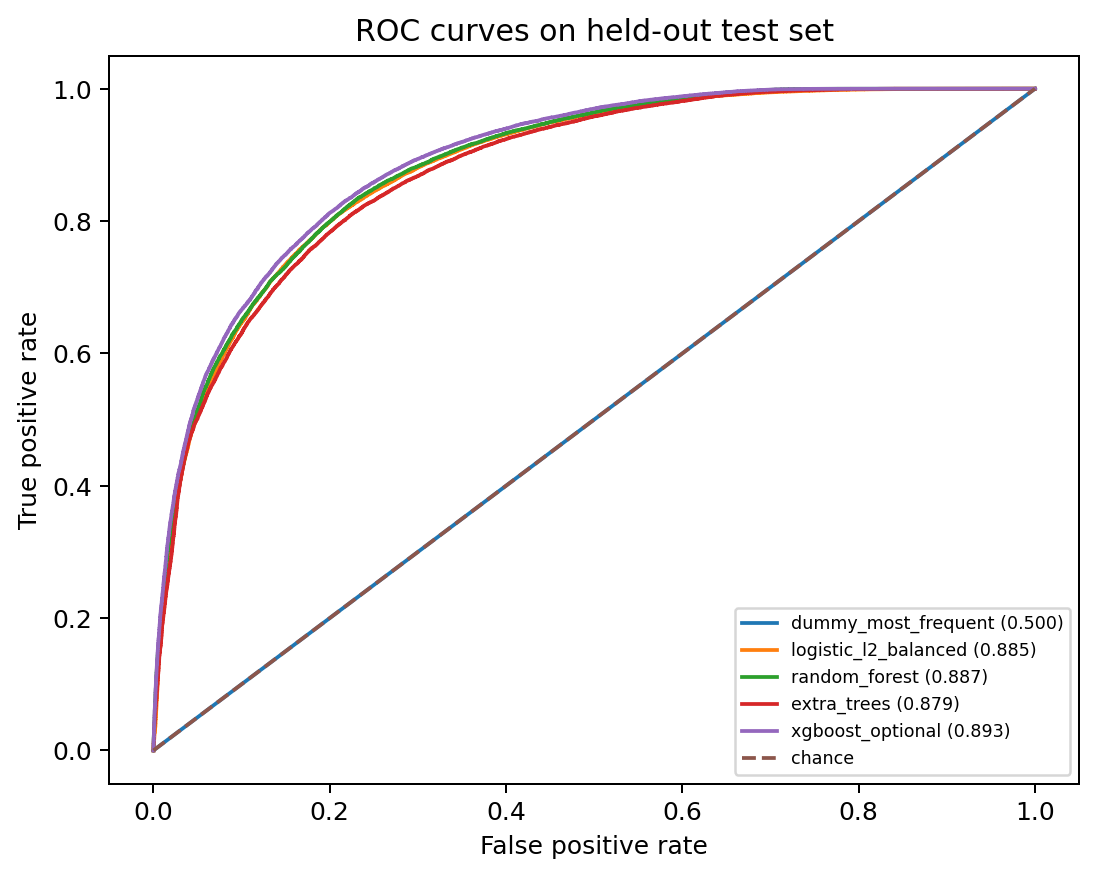
\includegraphics[width=0.48\linewidth]{figures/fig_roc_curves.png}
\caption{Precision-recall and ROC curves on the held-out 2025 test set. Learned models substantially outperform the dummy baseline, with XGBoost leading by PR-AUC.}
\end{figure}

The confusion matrix displays the tradeoff that was chosen for the F1 threshold. The best model indicates a preference for recall while maintaining precision at 0.74 or above. This is an appropriate choice for a safety-oriented project. However, the correct threshold would depend on the actual purpose of the project, which this project does not attempt to analyze.

\subsection{Ablation results}
An experiment involving the ablation of the linked tables can help establish whether the inclusion of those tables has provided any value to the model. The crash-only model achieved a PR-AUC of 0.656 and a ROC-AUC of 0.706. Including the vehicle aggregates increased the PR-AUC to 0.795. Including the person aggregates increased the PR-AUC to 0.830. Finally, including all features from the crash, vehicle, and person tables led to a PR-AUC of 0.846 and a ROC-AUC of 0.885. Thus, while this is the strongest evidence of the value of the tables in particular, these results also suggest that the vehicle and person files contributed something beyond the crash table’s features.

\begin{figure}[H]
\centering
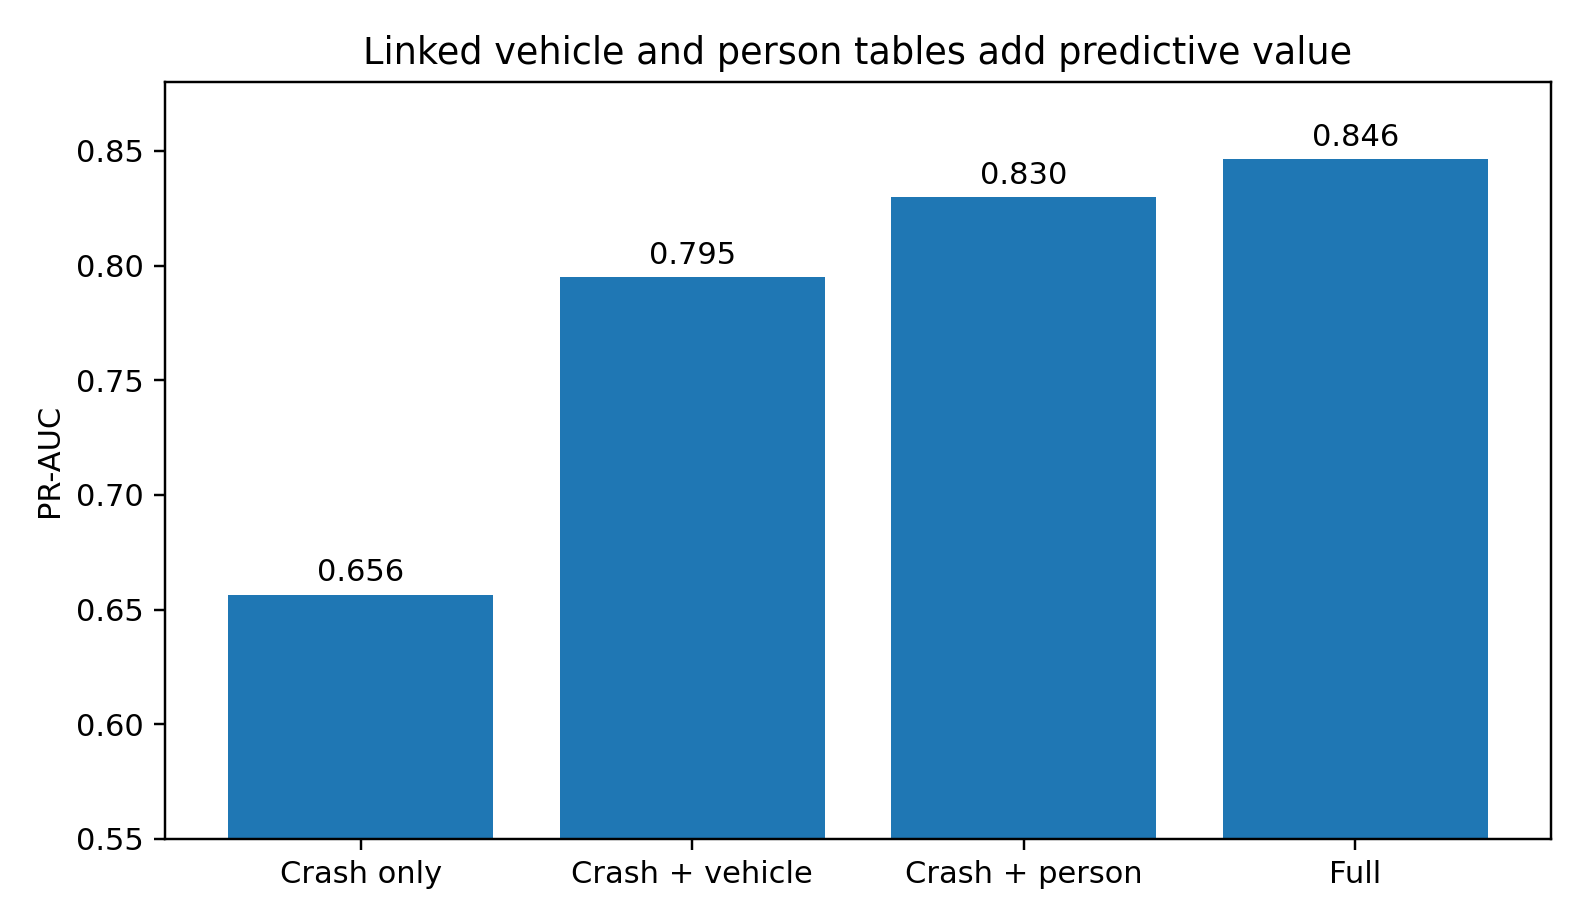
\includegraphics[width=0.70\linewidth]{figures/fig_ablation_pr_auc.png}
\caption{Feature-source ablation with logistic regression. Linked vehicle and person aggregates greatly improve PR-AUC over the crash-only model, and the full feature set performs best.}
\end{figure}

The most important feature for the best model was \texttt{person\_occupant\_share}. Other important features included variables related to the unknown driver sex share, whether the vehicle was parked prior to the crash, the contributing factors to the crash, the latitude of the crash, whether the vehicle was a motorcycle, the number of female persons within the vehicle, the number of persons involved in each role (driver, passenger, etc.), the borough in which the crash occurred, the number of persons wearing safety belts, the age of persons within the vehicle, the longitude of the crash, whether the vehicle was off of a street, the number of persons involved who were pedestrians, and the year in which the vehicle was made. Each of these variables should be interpreted only as variables that are associated with crashes occurring, and not as indicators of any causal relationship between those variables and traffic crashes.

\begin{figure}[H]
\centering
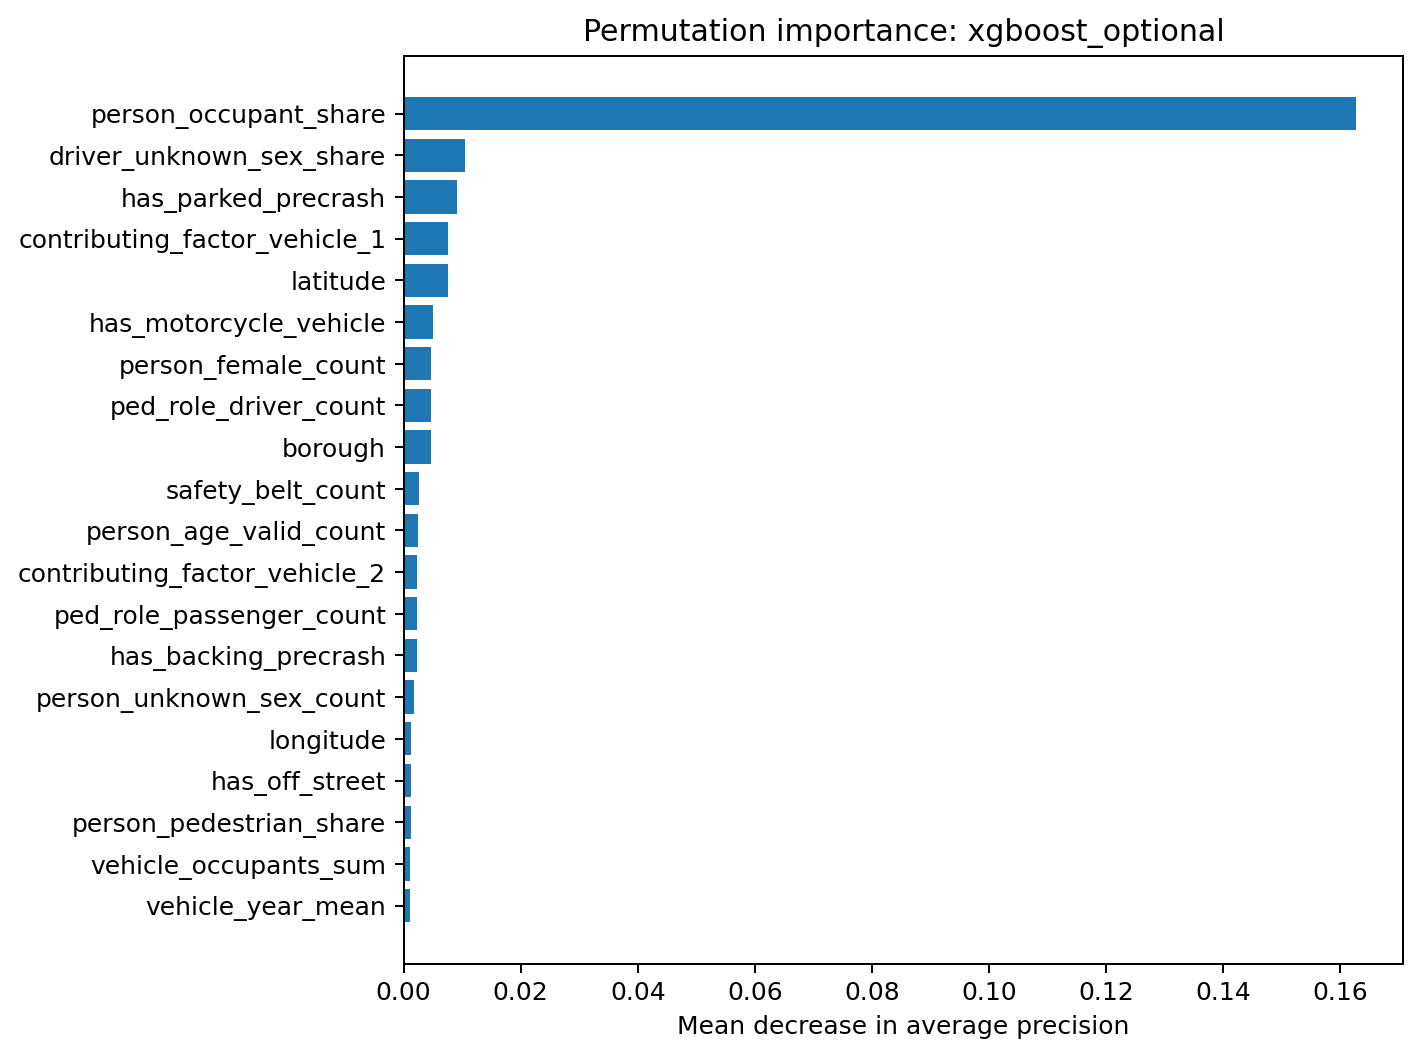
\includegraphics[width=0.48\linewidth]{figures/fig_feature_importance.png}\hfill
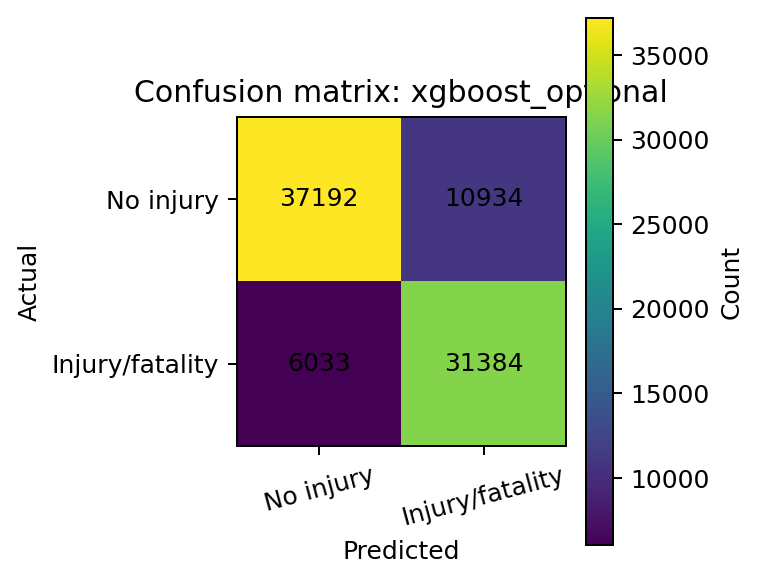
\includegraphics[width=0.48\linewidth]{figures/fig_confusion_matrix_best.png}
\caption{Interpretability and classification behavior. Left: permutation importance for the best model. Right: confusion matrix for XGBoost on the 2025 test set.}
\end{figure}

\section{Unsupervised crash archetypes}

The unsupervised method groups the 463 ZIP codes into groups according to the ZIP code groupings and computes summaries of collision characteristics within each group. Each vector for each group is standardized and transformed into two principal components \citep{jolliffe2016pca} which are then used to apply the K-Means clustering algorithm \citep{macqueen1967}. The silhouette algorithm determines that two clusters exist among the 61 groups of ZIP codes. The first two components of the principal component analysis explain 33.3 and 20.6 percent of the variance in the data, respectively.

The cluster with the most groups (designated Cluster 0) includes 53 of the groups and represents the more common profile for collision data. It has a higher average number of collisions within each group, a weekend share of approximately 26.6 percent, and a rush-hour share of 32.7 percent. Cluster 0 has lower shares of collisions involving bicycles, taxi vehicles, and pedestrians. Cluster 1 includes the remaining eight groups and has a lower average number of collisions within each group. It has a higher weekend and late-night share, a higher involvement of pedestrians and bicyclists, taxi vehicles, and bike-vehicle collisions. The injury rates for both clusters is similar at approximately 40.2 and 40.6 percent, respectively.

\begin{figure}[H]
\centering
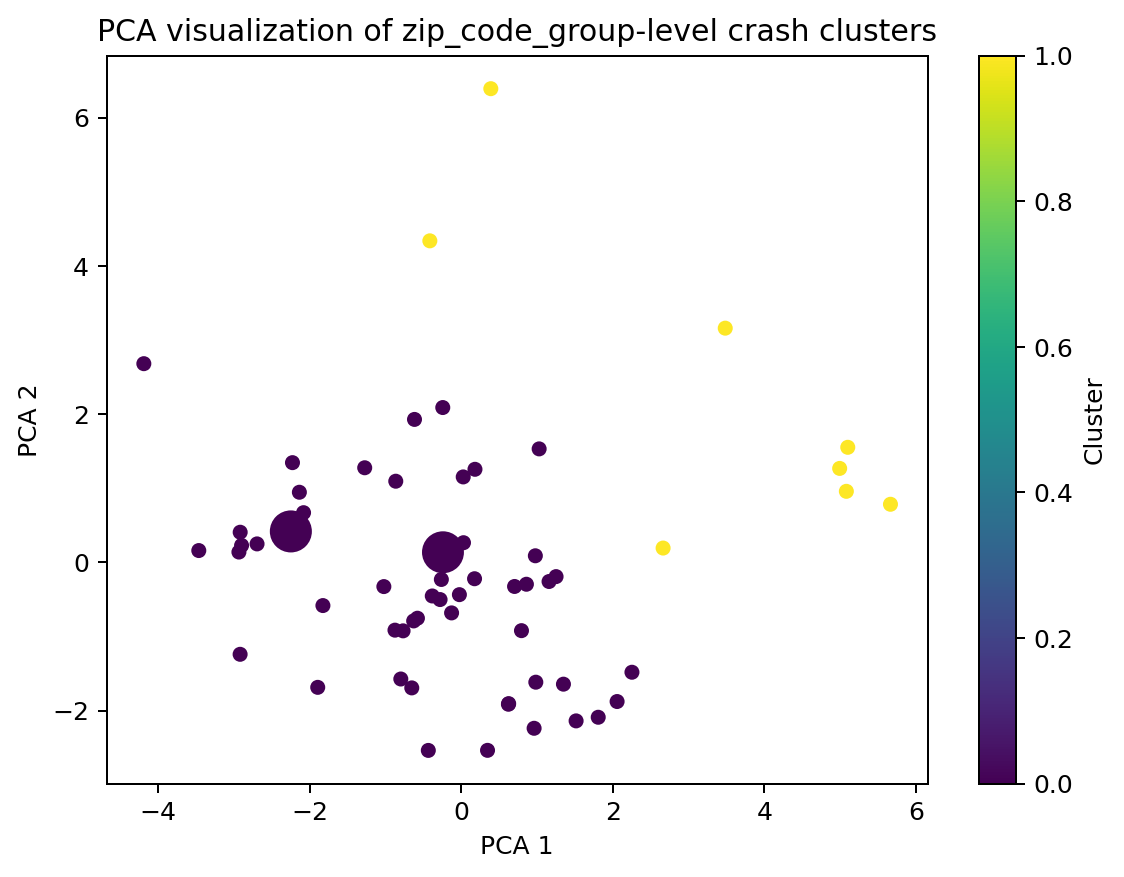
\includegraphics[width=0.48\linewidth]{figures/fig_pca_clusters.png}\hfill
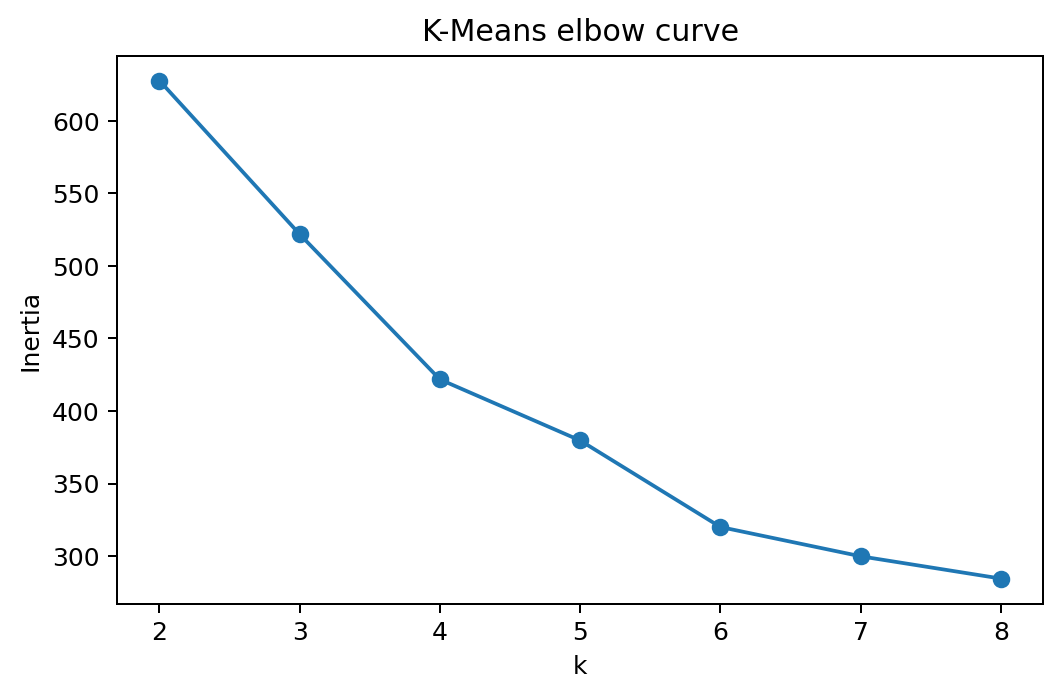
\includegraphics[width=0.48\linewidth]{figures/fig_kmeans_elbow.png}
\caption{Unsupervised geographic profiles. PCA visualization and K-Means diagnostics identify two broad ZIP-code group profiles that differ more in road-user mix and timing than in injury rate alone.}
\end{figure}

\section{Discussion}
The main finding is that injury-producing collisions can be reasonably well predicted from the available data. Such high scores for the PR-AUC and ROC-AUC metrics are not surprising, given the richness of the data available to us, but also due to the measures we have taken to ensure that there is no leakage in our models. The best performing models did not use any information about the injury of persons involved in the collisions or the number of injuries in each collision as any of the features for modeling. Instead, the models used information like the composition of the road users, the vehicles involved, the factors that contributed to each collision, and the geographical features of each of the collisions.

The ablation results are the most important results to discuss regarding this project. The crash-only model does contain some information that is useful for modeling the outcome, but the area under the PR-AUC curve is much lower than that of the model with all features. The vehicle aggregates contribute to the model because they reveal information about the vehicles that were involved in each collision. The person aggregates contribute to the model because they reveal information about the individuals involved in each of the collisions. The inclusion of these features improves the model because they contain information that is complementary to the features already within the collision and crash data set itself.

Beyond the ablation studies, these models can help to explore the collisions data in additional ways. The logistic regression model allows for the interpretation of the coefficients of the variables in the model. Additionally, the permutation importance values from the XGBoost models help to reveal information about which features had the most impact on the performance of the model. These interpretations, however, should not be treated as a means of establishing causation between these features and the binary outcome. For instance, the information about the borough in which the crashes occurred may be a means of capturing information about the volume of the road users in that area, the number of crashes that occur there, the characteristics of the residents that live in that area, or some other feature that is not directly observable from the crashes data itself. Similarly, the association between the count of persons involved in each collision and the label of whether those crashes resulted in injuries to those persons may be due to the fact that collisions that involve more persons will necessarily expose more persons to the risk of collisions, but does not necessarily indicate that this feature has any relationship to the outcomes itself.

\section{Limitations}
There are several limitations to the present analysis. First, the dataset is observational and administrative. It does not include all the collisions or near misses by police officers. Furthermore, according to the data repository, these data are preliminary and subject to change \citep{nyc_crashes}. Second, there are no exposure variables in the dataset. For instance, the dataset does not have variables representing the number of vehicles miles driven, the number of pedestrians, the number of bicycles, the road geometry, or the weather at each intersection. If there were such variables, it would be possible to determine whether the number of collisions with injury are actually related to the number of individuals that travel through each area.

Third, the values for some variables are only available after the crash report is completed by the police officers. In these cases, the model is retrospective rather than predictive of the number of collisions with injuries. Fourth, while great efforts were made to reduce the risk of leakage, it is not possible to eliminate all forms of leakage. For instance, fields like the contributing factor to the collision or the action of the drivers involved in the collision are reported by the police officers after the fact. Fifth, even with the use of the 2025 test set, which is better than using a random split of the data, it is still possible that the model would have performed differently with a split of the data from another year or with a different policy on the road in New York City.

\section{Reproducibility and compute}
The repository also contains the Python script, the requirements file, the README file, and the outputs of the analysis. These files were executed on a computer with Python 3.12.2 on Windows 10. The completed analysis took approximately 904.5 seconds to execute. The XGBoost and SHAP libraries were installed as optional packages. The other packages necessary to execute the analysis are pandas, NumPy, scikit-learn, matplotlib, scipy, and pyarrow. The raw CSV data files were not committed to the repository because of their large size and as public data files. However, the README file contains the names of the expected data files on the local machine and includes links to download the three data tables from NYC Open Data.

\section{Conclusion}
This project takes a crash data set with multiple tables and transforms it into a data science workflow for the prediction of injury-producing collisions in NYC. XGBoost fared the best in its predictive performance, though logistic regression was also competitive in its performance and interpretability. The ablation study indicated the value of using vehicle and person data in addition to the crash data itself. Finally, the clustering analysis revealed two main clusters of crashes in NYC according to their geographic location. The results of this project demonstrate the value of the techniques used in creating such a model and their relevance to the city of NYC, though remain limited in their conclusions to the detection of only the associations between variables.

\clearpage
\section*{References}
\small
\begin{thebibliography}{10}

\bibitem[Breiman(2001)]{breiman2001random}
Breiman, L. (2001). Random forests. \textit{Machine Learning}, 45(1):5-32.

\bibitem[Chen and Guestrin(2016)]{xgboost}
Chen, T. and Guestrin, C. (2016). XGBoost: A scalable tree boosting system. In \textit{Proceedings of the 22nd ACM SIGKDD International Conference on Knowledge Discovery and Data Mining}, pages 785-794.

\bibitem[City of New York(2026a)]{nyc_crashes}
City of New York. (2026a). Motor Vehicle Collisions - Crashes. \url{https://catalog.data.gov/dataset/motor-vehicle-collisions-crashes}. Accessed May 2026.

\bibitem[City of New York(2026b)]{nyc_vehicles}
City of New York. (2026b). Motor Vehicle Collisions - Vehicles. \url{https://catalog-beta.data.gov/dataset/motor-vehicle-collisions-vehicles}. Accessed May 2026.

\bibitem[City of New York(2026c)]{nyc_person}
City of New York. (2026c). Motor Vehicle Collisions - Person. \url{https://catalog.data.gov/dataset/motor-vehicle-collisions-person}. Accessed May 2026.

\bibitem[Jolliffe and Cadima(2016)]{jolliffe2016pca}
Jolliffe, I. T. and Cadima, J. (2016). Principal component analysis: A review and recent developments. \textit{Philosophical Transactions of the Royal Society A}, 374(2065).

\bibitem[MacQueen(1967)]{macqueen1967}
MacQueen, J. (1967). Some methods for classification and analysis of multivariate observations. In \textit{Proceedings of the Fifth Berkeley Symposium on Mathematical Statistics and Probability}, pages 281-297.

\bibitem[NYC DOT(2026)]{nyc_dot_2026}
New York City Department of Transportation. (2026). Traffic deaths reach all-time low: New York ends year with fewest fatalities ever recorded. \url{https://www.nyc.gov/html/dot/html/pr2026/traffic-deaths-reach-all-time-low.shtml}. Accessed May 2026.

\bibitem[Pedregosa et al.(2011)]{sklearn}
Pedregosa, F. et al. (2011). Scikit-learn: Machine learning in Python. \textit{Journal of Machine Learning Research}, 12:2825-2830.

\bibitem[Santos et al.(2022)]{santos2022review}
Santos, K., Dias, J. P., and Amado, C. (2022). A literature review of machine learning algorithms for crash injury severity prediction. \textit{Journal of Safety Research}, 80:254-269.

\end{thebibliography}

\end{document}
